\setcounter{ex}{0}
\section{PHƯƠNG TRÌNH LƯỢNG GIÁC}
% \subsection{Ví dụ minh hoạ}
% \Opensolutionfile{ans}[ans/DA-CD6-LUONG-GIAC-VD]
% \begin{vd}
%     Giải các phương trình lượng giác sau
%     \begin{listEX}[4]
%         \item $\sin x=1$
%         \item $2\cos x-\sqrt{3}=0$
%         \item $\tan x=\sqrt{2}$
%         \item $\tan x=\tan 3x$
%     \end{listEX}
%     \loigiai{
        
%     }
%     \dotlineEX{5}% Tạo các dòng kẻ trong tài liệu
% \end{vd}
% \begin{vd}
%     Vẽ đồ thị của các hàm số sau
%     \begin{listEX}[2]
%         \item $y=\sin x$\\
%         \begin{tikzpicture}[>=stealth, xscale=.55,yscale=1]
%             % 1. Vẽ lưới ô vuông phụ (mờ) để học sinh dễ căn tọa độ
%             % Mỗi ô vuông tương ứng với 0.5 đơn vị
%             \draw[color=gray!15, thin, step=0.5] (-7,-1.6) grid (7,1.6);
%             % 3. Vẽ hai trục tọa độ Ox, Oy
%             \draw[->, ultra thick] (-7.2,0) -- (7.2,0) node[below] {$x$};
%             \draw[->, ultra thick] (0,-1.5) -- (0,1.5) node[left] {$y$};
%             \node[below left] at (0,0) {$O$};
%             % 4. Đánh dấu các giá trị trên trục tung (y)
%             \foreach \y in {-1, 1}
%             \draw[thick] (2pt,\y) -- (-2pt,\y) node[left, scale=0.8] {$\y$};
%             \foreach \x/\l in {
%                 -6.28/-2\pi, -4.71/-\frac{3\pi}{2}, -3.14/-\pi, -1.57/-\frac{\pi}{2}, 
%                 1.57/\frac{\pi}{2}, 3.14/\pi, 4.71/\frac{3\pi}{2}, 6.28/2\pi
%             }
%             {
%                 \draw[thick] (\x,2pt) -- (\x,-2pt) node[below, scale=0.8, fill=white, inner sep=1pt, yshift=-2pt] {$\l$};
%             }
%         \end{tikzpicture}
%         \item $y=\cos x$\\
%         \begin{tikzpicture}[>=stealth, xscale=.55,yscale=1]
%             % 1. Vẽ lưới ô vuông phụ (mờ) để học sinh dễ căn tọa độ
%             % Mỗi ô vuông tương ứng với 0.5 đơn vị
%             \draw[color=gray!15, thin, step=0.5] (-7,-1.6) grid (7,1.6);
%             % 3. Vẽ hai trục tọa độ Ox, Oy
%             \draw[->, ultra thick] (-7.2,0) -- (7.2,0) node[below] {$x$};
%             \draw[->, ultra thick] (0,-1.5) -- (0,1.5) node[left] {$y$};
%             \node[below left] at (0,0) {$O$};
%             % 4. Đánh dấu các giá trị trên trục tung (y)
%             \foreach \y in {-1, 1}
%             \draw[thick] (2pt,\y) -- (-2pt,\y) node[left, scale=0.8] {$\y$};
%             \foreach \x/\l in {
%                 -6.28/-2\pi, -4.71/-\frac{3\pi}{2}, -3.14/-\pi, -1.57/-\frac{\pi}{2}, 
%                 1.57/\frac{\pi}{2}, 3.14/\pi, 4.71/\frac{3\pi}{2}, 6.28/2\pi
%             }
%             {
%                 \draw[thick] (\x,2pt) -- (\x,-2pt) node[below, scale=0.8, fill=white, inner sep=1pt, yshift=-2pt] {$\l$};
%             }
%         \end{tikzpicture}
%         \item $y=\tan x$\\
%         \begin{tikzpicture}[>=stealth, xscale=.55,yscale=1]
%             % 1. Vẽ lưới ô vuông phụ (mờ) để học sinh dễ căn tọa độ
%             % Mỗi ô vuông tương ứng với 0.5 đơn vị
%             \draw[color=gray!15, thin, step=0.5] (-7,-1.6) grid (7,1.6);
%             % 3. Vẽ hai trục tọa độ Ox, Oy
%             \draw[->, ultra thick] (-7.2,0) -- (7.2,0) node[below] {$x$};
%             \draw[->, ultra thick] (0,-1.5) -- (0,1.5) node[left] {$y$};
%             \node[below left] at (0,0) {$O$};
%             % 4. Đánh dấu các giá trị trên trục tung (y)
%             \foreach \y in {-1, 1}
%             \draw[thick] (2pt,\y) -- (-2pt,\y) node[left, scale=0.8] {$\y$};
%             \foreach \x/\l in {
%                 -6.28/-2\pi, -4.71/-\frac{3\pi}{2}, -3.14/-\pi, -1.57/-\frac{\pi}{2}, 
%                 1.57/\frac{\pi}{2}, 3.14/\pi, 4.71/\frac{3\pi}{2}, 6.28/2\pi
%             }
%             {
%                 \draw[thick] (\x,2pt) -- (\x,-2pt) node[below, scale=0.8, fill=white, inner sep=1pt, yshift=-2pt] {$\l$};
%             }
%         \end{tikzpicture}
%         \item $y=\cot x$\\
%         \begin{tikzpicture}[>=stealth, xscale=.55,yscale=1]
%             % 1. Vẽ lưới ô vuông phụ (mờ) để học sinh dễ căn tọa độ
%             % Mỗi ô vuông tương ứng với 0.5 đơn vị
%             \draw[color=gray!15, thin, step=0.5] (-7,-1.6) grid (7,1.6);
%             % 3. Vẽ hai trục tọa độ Ox, Oy
%             \draw[->, ultra thick] (-7.2,0) -- (7.2,0) node[below] {$x$};
%             \draw[->, ultra thick] (0,-1.5) -- (0,1.5) node[left] {$y$};
%             \node[below left] at (0,0) {$O$};
%             % 4. Đánh dấu các giá trị trên trục tung (y)
%             \foreach \y in {-1, 1}
%             \draw[thick] (2pt,\y) -- (-2pt,\y) node[left, scale=0.8] {$\y$};
%             \foreach \x/\l in {
%                 -6.28/-2\pi, -4.71/-\frac{3\pi}{2}, -3.14/-\pi, -1.57/-\frac{\pi}{2}, 
%                 1.57/\frac{\pi}{2}, 3.14/\pi, 4.71/\frac{3\pi}{2}, 6.28/2\pi
%             }
%             {
%                 \draw[thick] (\x,2pt) -- (\x,-2pt) node[below, scale=0.8, fill=white, inner sep=1pt, yshift=-2pt] {$\l$};
%             }
%         \end{tikzpicture}
%     \end{listEX}
% \end{vd}
% \begin{vd}
%     Tìm giá trị lớn nhất (GTLN) và giá trị nhỏ nhất (GTNN) của các hàm số sau:
%     \begin{listEX}[2]
%         \item $y = 4\sin x - 3$.
%         \item $y = 5 - 2\cos^2 x$.
%     \end{listEX}
%     \loigiai{
%         \begin{enumerate}
%             \item Xét hàm số $y = 4\sin x - 3$:
%             \begin{itemize}
%                 \item Ta có: $-1 \le \sin x \le 1, \forall x \in \mathbb{R}$.
%                 \item Nhân các vế với $4 > 0$, ta được: $-4 \le 4\sin x \le 4$.
%                 \item Cộng thêm $-3$ vào các vế: $-4 - 3 \le 4\sin x - 3 \le 4 - 3$.
%                 \item Suy ra: $-7 \le y \le 1$.
%             \end{itemize}
%             Vậy GTLN của hàm số là $M = 1$ khi $\sin x = 1$; GTNN của hàm số là $m = -7$ khi $\sin x = -1$.
            
%             \item Xét hàm số $y = 5 - 2\cos^2 x$:
%             \begin{itemize}
%                 \item Ta có: $0 \le \cos^2 x \le 1, \forall x \in \mathbb{R}$.
%                 \item Nhân các vế với $-2 < 0$, bất đẳng thức đổi chiều: $-2 \le -2\cos^2 x \le 0$.
%                 \item Cộng thêm $5$ vào các vế: $5 - 2 \le 5 - 2\cos^2 x \le 5 + 0$.
%                 \item Suy ra: $3 \le y \le 5$.
%             \end{itemize}
%             Vậy GTLN của hàm số là $M = 5$ khi $\cos x = 0$; GTNN của hàm số là $m = 3$ khi $\cos x = \pm 1$.
%         \end{enumerate}
%     }
% \end{vd}
% \Closesolutionfile{ans}
\subsection{Bài tập rèn luyện}
\Opensolutionfile{ans}[ans/DA-CD6-LUONG-GIAC-BTRL]
\begin{ex}[BGD-2025]
    Tập nghiệm của phương trình $\sin x = 0$ là
    \choice
    {$S = \left\{\dfrac{\pi}{2} + k\pi | k \in \mathbb{Z}\right\}$}
    {$S = \{k2\pi | k \in \mathbb{Z}\}$}
    {$S = \left\{\dfrac{\pi}{2} + k2\pi | k \in \mathbb{Z}\right\}$}
    {\True $S = \{k\pi | k \in \mathbb{Z}\}$}
    \loigiai{
        Phương trình cơ bản: $\sin x = 0 \Leftrightarrow x = k\pi, k \in \mathbb{Z}$.
    }
\end{ex}
\begin{ex}Nghiệm của phương trình $2 \sin x - 1 = 0$ là
    \choice
    {$x = \pm \dfrac{\pi}{3} + k2\pi, k \in \mathbb{Z}$}
    {$\left[ \begin{aligned} x &= \dfrac{\pi}{6} + k2\pi \\ x &= \dfrac{7\pi}{6} + k2\pi \end{aligned} \right. k \in \mathbb{Z}$}
    {\True $\left[ \begin{aligned} x &= \dfrac{\pi}{6} + k2\pi \\ x &= \dfrac{5\pi}{6} + k2\pi \end{aligned} \right. k \in \mathbb{Z}$}
    {$x = \pm \dfrac{\pi}{6} + k2\pi, k \in \mathbb{Z}$}
    \loigiai{
        Ta có $2 \sin x - 1 = 0 \Leftrightarrow \sin x = \dfrac{1}{2} = \sin \dfrac{\pi}{6}$. \\
        $\Leftrightarrow \left[ \begin{aligned} x &= \dfrac{\pi}{6} + k2\pi \\ x &= \pi - \dfrac{\pi}{6} + k2\pi \end{aligned} \right. \Leftrightarrow \left[ \begin{aligned} x &= \dfrac{\pi}{6} + k2\pi \\ x &= \dfrac{5\pi}{6} + k2\pi \end{aligned} \right., k \in \mathbb{Z}$.
    }
\end{ex}
\begin{ex}
    Tập nghiệm của phương trình $\cos x = 1$ là
    \choice
    {$S = \left\{\dfrac{\pi}{2} + k2\pi | k \in \mathbb{Z}\right\}$}
    {\True $S = \{k2\pi | k \in \mathbb{Z}\}$}
    {$S = \{k\pi | k \in \mathbb{Z}\}$}
    {$S = \left\{\dfrac{\pi}{2} + k\pi | k \in \mathbb{Z}\right\}$}
    \loigiai{
        Phương trình cơ bản: $\cos x = 1 \Leftrightarrow x = k2\pi, k \in \mathbb{Z}$.
    }
\end{ex}
\begin{ex}
    Phương trình $\cos x = -\dfrac{\sqrt{3}}{2}$ có tập nghiệm là
    \choice
    {$S=\left\{x = \pm \dfrac{\pi}{3} + k\pi; k \in \mathbb{Z}\right\}$}
    {$S=\left\{x = \pm \dfrac{\pi}{6} + k\pi; k \in \mathbb{Z}\right\}$}
    {\True $S=\left\{x = \pm \dfrac{5\pi}{6} + k2\pi; k \in \mathbb{Z}\right\}$}
    {$S=\left\{x = \pm \dfrac{\pi}{3} + k2\pi; k \in \mathbb{Z}\right\}$}
    \loigiai{
        $\cos x = -\dfrac{\sqrt{3}}{2} = \cos \dfrac{5\pi}{6} \Leftrightarrow x = \pm \dfrac{5\pi}{6} + k2\pi, (k \in \mathbb{Z})$.
    }
\end{ex}
\begin{ex}
    Giải phương trình $2 \cos x = 1$ được nghiệm là
    \choice
    {$S=\left\{ \dfrac{\pi}{3} + \dfrac{k\pi}{2}, k \in \mathbb{Z} \right\}$}
    {$S=\left\{ \dfrac{\pi}{3} + k\pi, k \in \mathbb{Z} \right\}$}
    {$S=\left\{ -\dfrac{\pi}{3} + \dfrac{k\pi}{3}, k \in \mathbb{Z} \right\}$}
    {\True $S=\left\{ \pm\dfrac{\pi}{3} + k2\pi, k \in \mathbb{Z} \right\}$}
%    \loigiai{
%        Ta có $2 \cos x = 1 \Leftrightarrow \cos x = \dfrac{1}{2} \Leftrightarrow x = \pm \dfrac{\pi}{3} + k2\pi, k \in \mathbb{Z}$.
%    }
\end{ex}
\begin{ex}[Phan Bội Châu lần 2-Nghệ An-2026]
    Cho $\cos x = \dfrac{1}{3}$. Tính giá trị của $\cos 2x$.
    \choice
    {$-\dfrac{8}{9}$}
    {$\dfrac{7}{9}$}
    {$\dfrac{8}{9}$}
    {\True $-\dfrac{7}{9}$}
    \loigiai{
        Ta có công thức nhân đôi: $\cos 2x = 2\cos^2 x - 1$. \\
        Thay $\cos x = \dfrac{1}{3}$ vào ta được: $\cos 2x = 2\left(\dfrac{1}{3}\right)^2 - 1 = \dfrac{2}{9} - 1 = -\dfrac{7}{9}$.
    }
\end{ex}
\begin{ex}[Chuyên Lê Thánh Tông-Đà Nẵng-2026]
    Tập nghiệm của phương trình $\tan x = 1$ là
    \choice
    {$S = \left\{\dfrac{k\pi}{4} | k \in \mathbb{Z}\right\}$}
    {$S = \left\{\dfrac{\pi}{3} + k\pi | k \in \mathbb{Z}\right\}$}
    {\True $S = \left\{\dfrac{\pi}{4} + k\pi | k \in \mathbb{Z}\right\}$}
    {$S = \left\{-\dfrac{\pi}{4} + k\pi | k \in \mathbb{Z}\right\}$}
    \loigiai{
        $\tan x = 1 \Leftrightarrow \tan x = \tan \frac{\pi}{4} \Leftrightarrow x = \dfrac{\pi}{4} + k\pi, k \in \mathbb{Z}$.
    }
\end{ex}
\begin{ex}[KSCL 12-Hà Nội-2026]
    Tập xác định của hàm số $y = \tan x$ là
    \choice
    {$\mathbb{R} \setminus \left\{\dfrac{\pi}{2} + k2\pi | k \in \mathbb{Z}\right\}$}
    {$\mathbb{R} \setminus \{k\pi | k \in \mathbb{Z}\}$}
    {$\mathbb{R} \setminus \{k2\pi | k \in \mathbb{Z}\}$}
    {\True $\mathbb{R} \setminus \left\{\dfrac{\pi}{2} + k\pi | k \in \mathbb{Z}\right\}$}
    \loigiai{
        Hàm số $y = \tan x = \dfrac{\sin x}{\cos x}$ xác định khi $\cos x \neq 0 \Leftrightarrow x \neq \dfrac{\pi}{2} + k\pi, k \in \mathbb{Z}$.
    }
\end{ex}
\begin{ex}%[1D1N5-2]
    Phương trình nào sau đây vô nghiệm?
    \choice
    {$ \cos x=-\dfrac{3}{7} $}
    {$ \tan\left(3x+\dfrac{\pi}{6}\right)=-2019$}
    {\True $ \sin 3x=\dfrac{2019}{2018} $}
    {$ \cot 2x=\dfrac{9}{5} $}
    \loigiai{
        Phương trình $ \sin 3x=\dfrac{2019}{2018} $ vô nghiệm do $ a=\dfrac{2019}{2018}>1 $.
    }
\end{ex}
\begin{ex} Phương trình $\cos x - m = 0$ vô nghiệm khi $m$ là
    \choice
    {\True $\left[ \begin{aligned} m &< -1 \\ m &> 1 \end{aligned} \right.$}
    {$m > 1$}
    {$-1 \le m \le 1$}
    {$m < -1$}
    \loigiai{
        Phương trình tương đương $\cos x = m$. \\
        Vì tập giá trị của hàm số $y = \cos x$ là $[-1; 1]$, nên phương trình vô nghiệm khi $|m| > 1 \Leftrightarrow \left[ \begin{aligned} m &< -1 \\ m &> 1 \end{aligned} \right.$.
    }
\end{ex}
\begin{ex}
    \immini[thm]{Đường cong trong hình vẽ dưới đây là đồ thị của hàm số nào trong bốn hàm số sau?\choice
        {$y = \sin x$}
        {\True $y = \cos x$}
        {$y = \tan x$}
        {$y = \cot x$}}{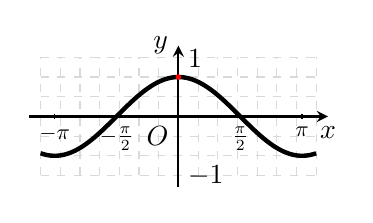
\begin{tikzpicture}[>=stealth,scale=.5]
            % Vẽ lưới mờ
            \draw[color=gray!30,dashed,step=0.5] (-3.5,-1.5) grid (3.5,1.5);
            % Vẽ trục tọa độ
            \draw[->,thick] (-3.8,0) -- (3.8,0) node[below] {$x$};
            \draw[->,thick] (0,-1.8) -- (0,1.8) node[left] {$y$};
            \node[below left] at (0,0) {$O$};
            % Vẽ đồ thị cos(x)
            \draw[ultra thick,black,samples=200,domain=-3.5:3.5] plot (\x,{cos(\x r)});
            % Điểm cực trị và nhãn
            \draw[dashed] (0,1) -- (0,1) node[above right] {$1$};
            \draw[dashed] (0,-1) -- (0,-1) node[below right] {$-1$};
            \fill[red] (0,1) circle (2pt);
            % Nhãn trục hoành
            \foreach \x/\label in {-3.14/-\pi, -1.57/-\frac{\pi}{2}, 1.57/\frac{\pi}{2}, 3.14/\pi}
            \draw (\x,2pt) -- (\x,-2pt) node[below,scale=0.8] {$\label$};
    \end{tikzpicture}}
\end{ex}
\begin{ex}
    Đồ thị hàm số $y = \tan x$ được biểu diễn bởi hình vẽ nào sau đây?
    \choice
    % Đáp án A: Sin (để nhiễu)
    {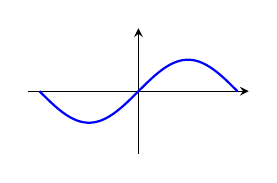
\begin{tikzpicture}[>=stealth,scale=0.4]
            \draw[->] (-3.5,0) -- (3.5,0); \draw[->] (0,-2) -- (0,2);
            \draw[thick,blue,samples=100,domain=-3.14:3.14] plot (\x,{sin(\x r)});
    \end{tikzpicture}}
    % Đáp án B: Cos (để nhiễu)
    {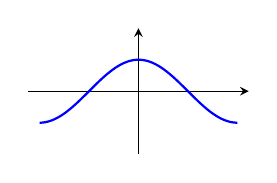
\begin{tikzpicture}[>=stealth,scale=0.4]
            \draw[->] (-3.5,0) -- (3.5,0); \draw[->] (0,-2) -- (0,2);
            \draw[thick,blue,samples=100,domain=-3.14:3.14] plot (\x,{cos(\x r)});
    \end{tikzpicture}}
    % Đáp án C: Tan (ĐÚNG)
    {\True 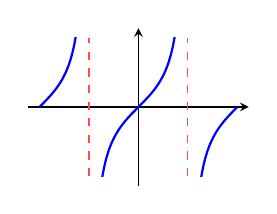
\begin{tikzpicture}[>=stealth,scale=0.4]
            \draw[->] (-3.5,0) -- (3.5,0); \draw[->] (0,-2.5) -- (0,2.5);
            % Giới hạn vùng vẽ để không bị vọt ra ngoài
            \begin{scope}
                \clip (-3.2,-2.2) rectangle (3.2,2.2);
                \draw[thick,blue,samples=100,domain=-1.35:1.35] plot (\x,{tan(\x r)});
                \draw[thick,blue,samples=100,domain=1.8:3.14] plot (\x,{tan(\x r)});
                \draw[thick,blue,samples=100,domain=-3.14:-1.8] plot (\x,{tan(\x r)});
            \end{scope}
            % Đường tiệm cận
            \draw[dashed,red!70] (1.57,-2.2) -- (1.57,2.2);
            \draw[dashed,red!70] (-1.57,-2.2) -- (-1.57,2.2);
    \end{tikzpicture}}
    % Đáp án D: Cot (để nhiễu)
    {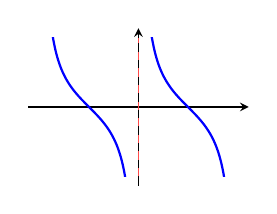
\begin{tikzpicture}[>=stealth,scale=0.4]
            \draw[->] (-3.5,0) -- (3.5,0); \draw[->] (0,-2.5) -- (0,2.5);
            \begin{scope}
                \clip (-3.2,-2.2) rectangle (3.2,2.2);
                \draw[thick,blue,samples=100,domain=0.3:2.8] plot (\x,{1/tan(\x r)});
                \draw[thick,blue,samples=100,domain=-2.8:-0.3] plot (\x,{1/tan(\x r)});
            \end{scope}
            \draw[dashed,red!70] (0,-2.2) -- (0,2.2);
    \end{tikzpicture}}
\end{ex}
\begin{ex}
    Tìm giá trị lớn nhất $M$ và giá trị nhỏ nhất $m$ của hàm số $y = 2\cos x$.
    \choice
    {\True $M = 2, m = -2$}
    {$M = 1, m = -1$}
    {$M = 2, m = 0$}
    {$M = 0, m = -2$}
    \loigiai{
        Ta có $-1 \le \cos x \le 1$ với mọi $x \in \mathbb{R}$. \\
        Nhân cả hai vế với $2 > 0$, ta được: \\
        $-2 \le 2\cos x \le 2$ \\
        $\Rightarrow -2 \le y \le 2$. \\
        Vậy $M = 2$ và $m = -2$.
    }
\end{ex}
\begin{ex}
    Tìm giá trị lớn nhất $M$ và giá trị nhỏ nhất $m$ của hàm số $y = 3\sin^2x + 2$.
    \choice
    {$M = 5, m = 1$}
    { $M = 5, m = -1$}
    {$M = 3, m = -3$}
    {\True$M = 5, m = 2$}
    \loigiai{
    }
\end{ex}
\begin{ex}
    Nghiệm lớn nhất của phương trình $2\cos 2x - 1 = 0$ trong đoạn $[0; \pi]$ là
    \choice
    {$x = \pi$}
    {$x = \dfrac{11\pi}{12}$}
    {$x = \dfrac{2\pi}{3}$}
    {\True $x = \dfrac{5\pi}{6}$}
    \loigiai{
        $2\cos 2x - 1 = 0 \Leftrightarrow \cos 2x = \dfrac{1}{2} \Leftrightarrow 2x = \pm \dfrac{\pi}{3} + k2\pi \Leftrightarrow x = \pm \dfrac{\pi}{6} + k\pi$. \\
        Các nghiệm trong $[0; \pi]$ là $\dfrac{\pi}{6}$ và $\dfrac{5\pi}{6}$. Nghiệm lớn nhất là $\dfrac{5\pi}{6}$.
    }
    \dotlineEX{1}% Tạo các dòng kẻ trong tài liệu
\end{ex}
\begin{ex}
    Số nghiệm thuộc khoảng $(0; 2\pi)$ của phương trình $\sin \left(x + \dfrac{\pi}{3}\right) + \sin 2x = 0$ là
    \choice
    {$1$}
    {$2$}
    {$3$}
    {\True $4$}
    \loigiai{
        $\sin \left(x + \dfrac{\pi}{3}\right) = \sin(-2x) \Leftrightarrow \left[\begin{aligned} &x + \frac{\pi}{3} = -2x + k2\pi \\ &x + \frac{\pi}{3} = \pi + 2x + k2\pi \end{aligned}\right. \Leftrightarrow \left[\begin{aligned} &x = -\frac{\pi}{9} + \frac{k2\pi}{3} \\ &x = -\frac{2\pi}{3} - k2\pi \end{aligned}\right.$ \\
        Trong $(0; 2\pi)$, các nghiệm là: $\dfrac{5\pi}{9}, \dfrac{11\pi}{9}, \dfrac{17\pi}{9}$ và $\dfrac{4\pi}{3}$. Tổng cộng có $4$ nghiệm.
    }
        \dotlineEX{1}% Tạo các dòng kẻ trong tài liệu
\end{ex}
\begin{ex}
    Số nghiệm của phương trình $\tan 3x - \tan x = 0$ trên nửa khoảng $[0; 2\pi)$ bằng
    \choice
    {$1$}
    {\True $2$}
    {$3$}
    {$4$}
    \loigiai{
        Điều kiện: $\cos 3x \neq 0$ và $\cos x \neq 0$. \\
        Phương trình $\Leftrightarrow \tan 3x = \tan x \Leftrightarrow 3x = x + k\pi \Leftrightarrow x = k\dfrac{\pi}{2}$. \\
        Trên $[0; 2\pi)$, ta có các giá trị $x \in \{0; \frac{\pi}{2}; \pi; \frac{3\pi}{2}\}$. \\
        Đối chiếu điều kiện, loại $x = \frac{\pi}{2}$ và $x = \frac{3\pi}{2}$ (làm $\cos x = 0$). \\
        Vậy còn 2 nghiệm là $x = 0, x = \pi$.
    }
        \dotlineEX{2}% Tạo các dòng kẻ trong tài liệu
\end{ex}
\begin{ex}
    Số giờ ánh sáng mặt trời của một thành phố A trong ngày thứ $t$ được cho bởi hàm số $d(t) = 3\sin \left[\dfrac{\pi}{182}(t - 80)\right] + 12$. Hỏi thành phố A có đúng 12 giờ ánh sáng vào ngày nào?
    \choice
    {\True Ngày thứ 80 và 262}
    {Ngày thứ 80}
    {Ngày thứ 171}
    {Ngày thứ 171 và 353}
    \loigiai{
        Yêu cầu bài toán: $d(t) = 12 \Leftrightarrow 3\sin \left[\dfrac{\pi}{182}(t - 80)\right] = 0 \Leftrightarrow \sin \left[\dfrac{\pi}{182}(t - 80)\right] = 0$. \\
        $\Leftrightarrow \dfrac{\pi}{182}(t - 80) = k\pi \Leftrightarrow t = 182k + 80$. \\
        Với $0 < t \le 365$: $k=0 \Rightarrow t=80$; $k=1 \Rightarrow t=262$.
    }
    \dotlineEX{3}% Tạo các dòng kẻ trong tài liệu
\end{ex}
\begin{ex}
    Số giờ có ánh sáng mặt trời của Đà Nẵng năm 2023 được cho bởi $y = 3\sin \left[\dfrac{\pi}{180}(x + 60)\right] + 14$ với $x$ là ngày trong năm. Ngày nào số giờ ánh sáng lớn nhất?
    \choice
    {\True 30/01}
    {29/01}
    {31/01}
    {30/03}
    \loigiai{
        Số giờ ánh sáng lớn nhất khi $\sin \left[\dfrac{\pi}{180}(x + 60)\right] = 1 \Leftrightarrow \dfrac{\pi}{180}(x + 60) = \dfrac{\pi}{2} + k2\pi$. \\
        $\Leftrightarrow x + 60 = 90 + 360k \Leftrightarrow x = 30 + 360k$. \\
        Với $1 \le x \le 365$, chọn $k=0 \Rightarrow x=30$. Ngày thứ 30 của năm 2023 là ngày 30/01.
    }
    \dotlineEX{4}
\end{ex}
\begin{ex}
    Giả sử một vật dao động điều hòa theo phương trình $x = 2\cos \left(2\pi t - \dfrac{\pi}{3}\right)$. Trong thời gian từ 0 đến 5 giây, vật đi qua vị trí cân bằng bao nhiêu lần?
    \choice
    {$9$}
    {\True $10$}
    {$11$}
    {$12$}
    \loigiai{
        Vị trí cân bằng ứng với $x = 0 \Leftrightarrow \cos \left(2\pi t - \dfrac{\pi}{3}\right) = 0 \Leftrightarrow 2\pi t - \dfrac{\pi}{3} = \dfrac{\pi}{2} + k\pi \Leftrightarrow t = \dfrac{5}{12} + \dfrac{k}{2}$. \\
        Xét $0 \le \dfrac{5}{12} + \dfrac{k}{2} \le 5 \Leftrightarrow -\dfrac{5}{6} \le k \le \dfrac{55}{6} \approx 9{,}16$. \\
        Vì $k \in \mathbb{Z} \Rightarrow k \in \{0; 1; \dots; 9\}$, tổng cộng có 10 giá trị.
    }
    \dotlineEX{5}
\end{ex}
\Closesolutionfile{ans}